\documentclass{article}
\usepackage[utf8]{inputenc}
\usepackage[a4paper, portrait, margin=1in]{geometry}
\usepackage{tabularx}
\usepackage{graphicx}
\usepackage{amsmath}
\usepackage{hyperref}
\hypersetup{
    colorlinks=true,
    linkcolor=blue,
    filecolor=magenta,      
    urlcolor=cyan,
}


\title{OOAD \& Software Engineering (UE18CS353) \\
    Unit 4}
\author{Aronya Baksy}
\date{April 2021}

\begin{document}
\maketitle
\section{Software Testing}
\begin{itemize}
    \item Testing is executing software in a simulated or real environment, using inputs selected somehow
    
    \item Inadequate/incomplete testing leads to catastrophes (Therac-25, Ariane-5 etc.)
    
    \item In a normal waterfall model, testing activity follows the Requirement, Design, Implementation phases. This causes \textbf{large costs} in fixing errors and very late detection due to the big-bang nature of the testing
    
    \item In a V model, the testing is planned along with the corresponding SDLC phase. This results in better chance of picking up errors early and fixing them with minimal cost.
    
    \item In an Agile approach like Scrum:
    \begin{itemize}
        \item The entire team takes part in the entire test activity: test planning, test specification, test execution, test evaluation and result reporting 
        
        \item Each sprint involves creating unit tests for the code written in that sprint. These unit tests are created and run by the developers.
        
        \item Testers are in charge of testing functional and non functional attributes
        
        \item The customer carries out the User Acceptance test at the end of the sprint. The feedback from this test is used as input to the next sprint. 
        
        \item Test results are collected and maintained at the end of each sprint.
    \end{itemize}
\end{itemize}

\subsection{Objectives of Testing}
\begin{itemize}
    \item \textbf{Demonstration}: System can be used with acceptable risk level, in special conditions, and is ready for integration
    
    \item \textbf{Detection}: of defects, errors, and deficiencies. Determine quality of components and the overall system (capabilites and limitations)
    
    \item \textbf{Prevention}: of errors and defects being propagated to later stages. Clarify non-functional requirements, 
\end{itemize}

\subsection{Validation and Verification}
\begin{tabular}{|p{0.45\textwidth}|p{0.45\textwidth}|}
    \hline
    \textbf{Validation} & \textbf{Verification} \\
    \hline
    The assurance that a product, service, or system meets the needs of the customer and other identified stakeholders. & The evaluation of whether or not a product, service, or system complies with a regulation, requirement, specification, or imposed condition.  \\
    \hline
    Done via dynamic testing (execution of code) & Done using static testing \\
    \hline
    Target the capabilities and features defined in the projects scope and requirements definition & Targets on software architecture, design \\
    \hline
\end{tabular}

\subsection{Terminologies}
\begin{itemize}
    \item \textbf{Defect}: deviation from requirements. Imperfection due to design or coding mistake
    
    \item \textbf{Bug}: Programmer error that prevents correct operation of the system. 
    
    \item \textbf{Failure}: The state of the system that is caused by a defect. Occurs during development or later, and leads to unfulfillment of the requirements
    
    \item \textbf{Issue}: Raised by the end user when deployed product does not meet functional or non-functional requirements. Tracked using software like Jira
\end{itemize}

\section{Testing Types}
\subsection{Black-Box Testing (Functional Testing)}
\begin{itemize}
    \item Software is treated as a black box, no knowledge of internal implementation or logic. 
    
    \item Objective is to identify invalid outputs when valid or invalid inputs are given to the system. 
    
    \item Rqquires generated test cases to be passed to tester who executes the test cases on the system. 
    
    \item \textbf{Advantage}: early test planning, best for large units of code
    
    \item \textbf{Drawbacks}: Path coverage not good, hard to direct tests towards error-prone code
\end{itemize}

\subsection{White-Box Testing (Structural Testing)}
\begin{itemize}
    \item Factor in the logic and structure of the code. 
    
    \item Test cases derived using the knowledge of the above. Hence test cases are not made until implementation is complete
    
    \item \textbf{Advantages}: reveals hidden errors, partitioning by equivalence
    
    \item \textbf{Drawbacks}: testers need to have programming skills, hard to test all code (for large units)
\end{itemize}

\subsection{Grey-Box Testing}
\begin{itemize}
    \item Mix of functional and structural testing. 
    
    \item Test cases are designed using white-box methodology, but actual testing is done at the user level (black-box method)
    
    \item Can be used for integration testing between modules
\end{itemize}

\subsection{Static Testing}
\begin{itemize}
    \item Testing that does not involve any execution of code. 
    
    \item Carried out early on in the development stage, find errors and correct them as early as possible
    
    \item Static testing involves:
    \begin{itemize}
        \item Evaluation of code quality
        \item Data Flow
        \item Control Flow
        \item Cyclomatic Complexity
    \end{itemize}
\end{itemize}

\subsection{Dynamic Testing}
\begin{itemize}
    \item Involves running code to analyze the dynamic behaviour of the program under test. 
    
    \item Involves running the program with inputs and analyzing the outputs.
    
    \item Can find difficult and complex defects which are not easily detectable by static testing. 
    
    \item Types of dynamic testing:
    \begin{itemize}
        \item Testing based on techniques like Code based or Fault based
        
        \item Testing based on how the testing is done (Manual or Automatic)
        
        \item Testing based on different levels of testing (unit, integration, system, acceptance)
    \end{itemize}
\end{itemize}

\subsection{Based on Testing Technique}
\subsubsection{Control-Flow based Testing}
\begin{itemize}
    \item A control-flow path (aka a control-flow graph) is a representation of the logical structure of the program, in terms of the paths taken by a running program 
    
    \item Metrics: branch coverage of the test cases
\end{itemize}

\subsubsection{Data-Flow based Testing}
\begin{itemize}
    \item Finds paths in program based on location of definition and use of data variables in the program.
    
    \item Finds anomalies such as use without declaration, declaration without use, multiple declaration, deallocation without use etc.
\end{itemize}

\subsubsection{Error based Testing}
\begin{itemize}
    \item Use prior experience and domain knowledge to identify most common faults in the program
    
    \item Then design test cases to attack those faults and evaluate. 
\end{itemize}

\subsubsection{Fault based Testing}
\begin{itemize}
    \item Introduce faults into the code on purpose
    
    \item May lead to other faults being detected. Ideal outcome is that all test cases designed for correct program should fail on this new program.
\end{itemize}

\subsubsection{Mutation Testing}
\begin{itemize}
    \item Select certain statements (could be branch, arithmetic etc.) and make mutations on those. 
    
    \item Run all the tests against the mutants and the original. All mutants should fail 
    
    \item Reveals complex faults
\end{itemize}

\subsubsection{Specification based Testing}
\begin{itemize}
    \item Test output given an input strictly according to requirements laid out in the SRS
\end{itemize}

\subsubsection{Intuition based, Usage based, Domain based}
\begin{itemize}
    \item Based on the tester's intuition, the real world use cases and the application domain knowledge to design test cases
\end{itemize}

\subsection{Manual vs Automated Testing}
\subsubsection{Manual Testing}
\begin{itemize}
    \item Human performs tests without any test scripts or additional helpers
    
    \item Used for complex tests where automation is expensive
    
    \item Slow, tedious, low coverage
\end{itemize}
\subsubsection{Automated Testing}
\begin{itemize}
    \item Use test automation frameworks and test scripts to run tests with minimal human intervention
    
    \item Fast and repeatable but requires extra time for writing test scripts and framework maintenance.
    
    \item Efficient for periodic regular tests
\end{itemize}

\section{Testing Levels}
\subsection{Unit Testing}
\begin{itemize}
    \item Test smallest individually executable units of code. Check for coding or construction errors. 
    
    \item Unit test focussed on Algos and DS, interfaces, boundary conditions, error handling
    
    \item For OO projects this can be at the class level or at the method level
\end{itemize}

\subsection{Integration Testing}
\begin{itemize}
    \item Verify interfaces between components against the high-level design. Done by programmers
    
    \item Identify resource contention and timing problems that are not detected by unit tests. 
    
    \item Integration test strategies:
    \begin{itemize}
        \item \textbf{Big Bang}: integrate all modules and then check if system is running
        
        \item \textbf{Top-Down}: Simulate behaviour of lower level modules that are incomplete, using stubs. Integrate high level modules first then work downwards, in a depth-first manner. 
        
        \item \textbf{Bottom-Up}: Lowest level components are tested first, then used to facilitate the testing of higher level components (repeat until entire hierarchy is covered)
    \end{itemize}
\end{itemize} 

\subsection{System Testing}
\begin{itemize}
    \item Verify that a completely integrated system meets the requirements. Fix defects in system as a whole, as well as interfaces b/w components.
    
    \item Requirements are defined by an SRS or an FRS (Functional Req. Spec.) document 
    
    \item Varieties of system testing:
    \begin{itemize}
        \item Regression testing: test whether changes cause side effects
        
        \item Installation testing
        
        \item Startup/shutdown testing
        
        \item Load/Stress testing
        
        \item Platform testing (for cross-platform apps)
        
        \item Localization testing (does the app work across different locales of the world)
        
        \item Functional and non-functional testing 
    \end{itemize}
\end{itemize}

\subsection{Acceptance Testing}
\begin{itemize}
    \item Run test suite on complete system. Each test case in the suite includes a particular operating condition or use case in the real world. 
    
    \item Test environment is designed to be as close as possible to real world user. 
    
    \item Created by analysts, test engineers, customers and developers. Vital to include business logic tests as well as UI validation tests. 
    
    \item In an Agile methodology, an acceptance test case is similar to a single user story being played out. 
    
    \item Provide confidence that system meets business requirements. Acts as final gateway in terms of release, and contractual obligation between stakeholder and client. 
    
    \item The software can even be given to a small set of representative users for testing.
    \begin{itemize}
        \item In $\alpha$-testing, the group of test users test the product within the confined environment of the development group
        
        \item In $\beta$-testing, the group of test users test the product in the outside world. 
    \end{itemize}
\end{itemize}

\section{Test Planning and Strategy}
\begin{itemize}
    \item Test planning is the process of evolving a software test plan which discusses what, when and how testing has to be done as part of the project to ensure quality expectations can be met. 
    
    \item Test planning involves the following 9 activities:
\end{itemize}

\subsection{Define context and scope}
\begin{itemize}
    \item Review use case scenarios, discussions with developers and designers
    
    \item Review the documentation, perform a product walk-through
    
    \item Scope of testing is decided by customer requirements (domain, risk, quality), budget and schedule constraints, skills available in the test team.
\end{itemize}

\subsection{Define test adequacy criteria}
\begin{itemize}
    \item Criteria that determine when to stop testing i.e. consider testing to be complete for an iteration or sprint. 
    
    \item Based on code coverage criteria (lines of code, branch coverage etc.) or based on percentage of defects covered. 
\end{itemize}

\subsection{Test Strategy}
\begin{itemize}
    \item Test model, test types, test automation, test environment, and risk analysis + contingency planning come under test strategy
\end{itemize}

\subsubsection{Test Models/Mindsets}
\begin{itemize}
    \item \textbf{Demonstration Model}: whether the software runs successfully and passes the test cases designed for it. May lead to unconscious bias where only successful cases are tested  
    
    \item \textbf{Evaluation Model}: Focus on analysis and review techniques to detect faults in requirements and design documents
    
    \item \textbf{Destruction Model}: try to find as many faults in the program as possible. Difficult to decide adequacy because number of remaining faults is never known.
    
    \item \textbf{Preventive Model}: Prevent faults as early as possible with careful design, planning of test activity. 
\end{itemize}

\subsubsection{Test Type Chosen}
\begin{itemize}
    \item Each life cycle phase has testable outcomes 
    
    \item Start by low-level testing of small components and move towards integration into larger components. 
\end{itemize}

\subsubsection{Test Environment}
\begin{itemize}
    \item Software or hardware setup designed for testers to be able to execute their test cases. 
    
    \item Consists of the application under test, the server OS, test data, Database, front end for testing, servers/storage/network and documentation needed.
    
    \item Test environment needs to be maintained and managed, may involve periodic upgrades to keep the environment working.
    
    \item Challenges: planning, resource usage, remote environments, setup time and cost, sharing challenges, configuration
\end{itemize}

\subsubsection{Automation Strategy}
\begin{itemize}
    \item Define goals, plan test approach
    
    \item Select automation framework and test tool
    
    \item Develop test cases, then code test scripts. Execution of test cases
\end{itemize}

\subsubsection{Testing Tools}
\begin{itemize}
    \item Criteria for selection:
    \begin{itemize}
        \item Compatibility between application under test, and testing tool to be used
        
        \item Proficiency of testers in the selected tool, for best utilization
        
        \item Balance between features offered, test report detail generated, ease of use. 
        
        \item Cross-platform support
        
        \item Acceptance/popularity as an indication of available support and documentation
        
        \item Cost
    \end{itemize}
\end{itemize}

\subsubsection{Risk Analysis}
\begin{itemize}
    \item Risks in terms of:
    \begin{itemize}
        \item Changes in business/technology goals and competition
        
        \item Resource available
        
        \item Quality of product, test types/models not usable
        
        \item Test automation and tool problems
    \end{itemize}
\end{itemize}

\subsection{Deliverable List}
\begin{itemize}
    \item Most commonly, in the form of a list of test cases, and test specifications for each module. 
\end{itemize}

\subsection{Test Schedule Creation}
\begin{itemize}
    \item Create a WBS for the testing activites, using estimation techniques such as CoCoMo and others. 
    
    \item Includes estimation for building test strategy/specification/test cases/test environment setup and test execution, test reporting etc.)
\end{itemize}

\subsection{Planning, Identifying, Allocating Resources}
\begin{itemize}
    \item Test resource allocation between different teams in terms of hardware (servers/network/storage) and software (tools) 
    
    \item Identifying resources available, number and type of people working on project, and finally test environment and data needed by each team.
    
    \item Done in conjunction with the scheduling activity. 
\end{itemize}

\subsection{Identify milestones and risks}
\begin{itemize}
    \item Identify milestones in terms of resource allocation and the modified schedule. 
    
    \item Risks for completion of each of the task from a schedule and quality perspective is identified, analyzed, mitigation plans made and the triggers for kick-off identified.
    
    \item Milestones are used to track budget and schedule overruns, as well as identify risk triggers and mitigation plans. 
\end{itemize}

\subsection{Identify measures and metrics}
\begin{itemize}
    \item Measures:
    \begin{enumerate}
        \item The number of test cases planned and created
        \item Number of test cases run
        \item Time spent on creation, execution
        \item the number of errors found 
    \end{enumerate}
    
    \item Metrics:
    \begin{enumerate}
        \item Test cases executed per day
        
        \item Issues per kLoC, crititcal issues per kLoC
        
        \item Number of requirements traced over the lifecycle
    \end{enumerate}
\end{itemize}

\section{Test Process}
\begin{itemize}
    \item \textbf{Planning and control}: test strategy, adequacy criteria, schedule, review+approval boards
    \item \textbf{Analysis and Design}: Test requirements and product architecture
    \item \textbf{Implementation and execution}: design and run test cases, collect metrics and log results
    \item \textbf{Evaluate exit criteria and report}: Set up test stopping criteria 
    \item \textbf{Closure}: Verify all planned activities done, archive all config items created during testing
\end{itemize}

\section{Roles in testing}
\begin{itemize}
    \item \textbf{Director}: Oversight, co-ordination, high level vision and primary contact for clients and stakeholders to connect
    
    \item \textbf{Test Manager}: Prepare test plan and test strategy, monitor and control the test process
    
    \item \textbf{Infra Manager}: Manage all test infrastructure, capacity/maintenance and configuration support
    
    \item \textbf{Automation Manager}: Manage development/selection of testing tools and scripts
    
    \item \textbf{Test Architect}: Design test infrastructure, select/drive requirements for testing tools, validate the test strategy.
    
    \item \textbf{Test Analyst}: Maps customer environment and requirements to test environment and documentation
    
    \item \textbf{Test Engineer}: Carries out tests according to the methodology, plan and strategy developed. 
    
    \item \textbf{Test Development Engineer}: Develops scripts, tools for testing
\end{itemize}

\section{Test Metrics and Measurements}
\begin{itemize}
    \item Metric: a quantitative measure of the testing process indicating the progress, quality, productivity and the degree to which a system, possesses a given attribute. 
    
    \item Metrics must be understandable, quantitative, applicable, repeatable, economical to compute and language independent.
\end{itemize}
\subsection{Test Measures}
\begin{itemize}
    \item Size in LOC
    
    \item Fault density: bug per kLoC
    
    \item MTBF and its inverse, failure rate
    
    \item Defect distribution across SDLC phases, and across modules
    
    \item Defect leakage:
    \begin{equation*}
        Leakage = \frac{\text{\# of defects found in UAT}}{\text{\# of defects found before UAT}} \times 100
    \end{equation*}
    
    \item Test coverage: statement, branch, condition, loop, path, data flow coverage etc.
    
    \item Percent of tests executed and defects completed. 
    
    \item Defect discovery rate
    
    \item Percent injected faults discovered, mutation score: percent of mutants killed per total number of mutations introduced.
\end{itemize}
\begin{figure}[!h]
    \centering
    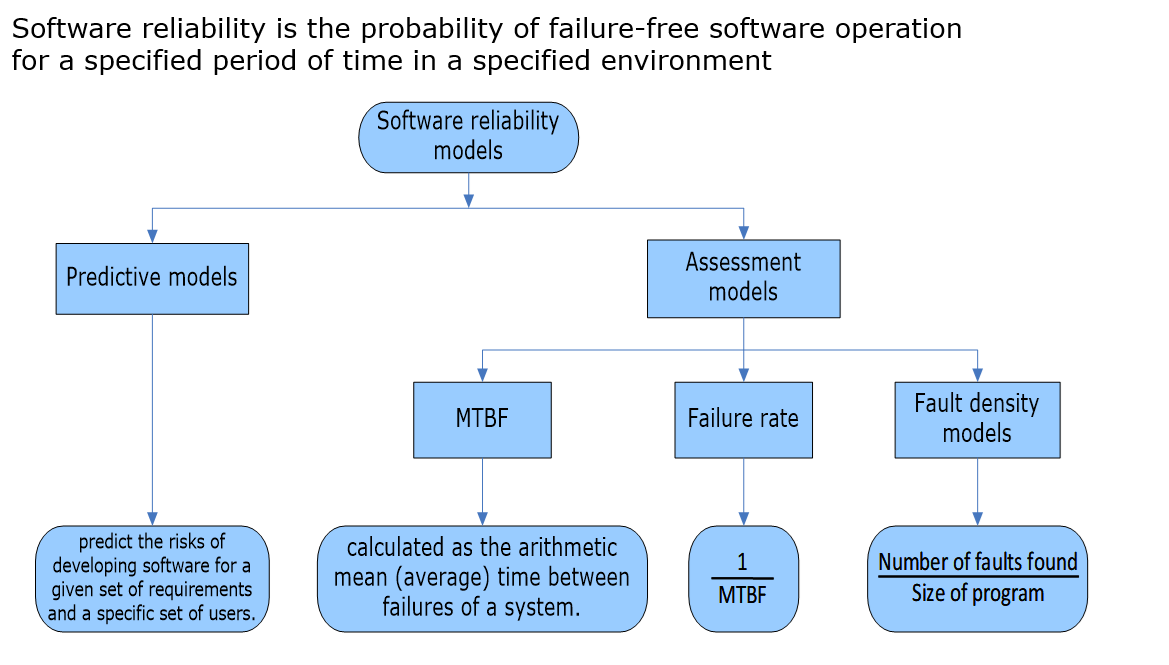
\includegraphics[scale=0.5]{p1.png}
    \caption{Test Reliability}
    \label{fig:my_label}
\end{figure}
\section{Software Maintenance}
\begin{itemize}
    \item The sustaining process of modifying a software system or component after delivery to correct faults, improve performance or other attributes, or adapt to a changed environment 
    
    \item Fixing defects from real-world use, fixing requirement and design defects, feature and performance enhancements, reaction to environmental changes, interfacing with other systems and retiring legacy components.
    
    \item Maintenance activities:
    \begin{itemize}
        \item Control over daily functioning, modifications to software
        
        \item Maintain performance at acceptable level
        
        \item Bug removal from existing software
    \end{itemize}
    
    \item Maintenance Drivers:
    \begin{itemize}
        \item Understanding of product from documentation
        
        \item Look at present and the change request at hand, to identify how to satisfy the task at hand
        
        \item Analyze the consequences of the solution as to how it affects any other future maintenance
    \end{itemize}
\end{itemize}
\subsection{Types}
\begin{itemize}
    \item \textbf{Predictive}: Modification after delivery to detect latent faults and correct them before they are exposed in production
    
    \item \textbf{Perfective}: Modification after delivery to improve performance or maintainability
    
    \item \textbf{Corrective}: Correction of detected faults post delivery
    
    \item \textbf{Adaptive}: Keep a product usable after delivery in response to changing environment

\end{itemize}

\subsection{Issues in maintenance}
\begin{itemize}
    \item \textbf{Technical}: caused by limitations in code/documentation quality, limited understanding of the project and lack of well-defined change scope 
    
    \item \textbf{Management}: Maintain people with high skill, align with economic objectives (due to lack of direct RoI from maintenance)
    
    \item \textbf{Outsourcing} of maintenance leads to challenges like IP protection, lack of control over process of development, learning curve
    
    \item \textbf{Costs} of staff availability, lifetime of project, contracts 
    
    \item \textbf{Predictability}: schedule, time alloted for maintenance.
\end{itemize}

\subsection{Maintenance Activities}
\subsubsection{Process Implementation}
\begin{itemize}
    \item Develop, document, and execute maintenance process plans including usage of tools as part of the maintenance process 
    
    \item Includes procedures for handling user reports and modification requests, issue tracking, response to user
\end{itemize}

\subsubsection{SMLC}
\begin{itemize}
    \item Identify problem
    
    \item Analyze the problem
    
    \item Open formal modification request and get it approved
    
    \item Design the change (modification to documentation and design)
    
    \item Implement the change
    
    \item Unit-test the change
    
    \item System test, regression test, acceptance test
    
    \item Delivery of the changed product as a patch. 
\end{itemize}

\subsubsection{Migration}
\begin{itemize}
    \item From old version to patched version of a product
    
    \item Migration plan involves:
    \begin{itemize}
        \item Notifying the user
        
        \item Applying the patch using restart or no restart (depends on kind of patch)
        
        \item White papers/tools used for more elaborate products
        
        \item Verify the process, support old data based on agreements
    \end{itemize}
\end{itemize}

\subsubsection{Retirement}
\begin{itemize}
    \item Retirement planning involves a timeline and methods for maintaining old data as needed
    
    \item Dispose ageing hardware and associated licenses and contracts
\end{itemize}

\subsection{Reverse Engineering and re-engineering}
\begin{itemize}
    \item \textbf{Reverse engineering} generates an alternate representation of the software apart from the existing code and documentation. 
    
    \item Allows maintainers to diagnose faults in components/their interfaces, without modifying/creating any product. 
    
    \item \textbf{Re-engineering} is hte process of modifying software to make it more understandable, and extensible. 
    
    \item Done only when standard maintenance techniques are not feasible or economical anymore. 
    
    \item May include refactoring, expected to improve CPU + memory untilization, and readability. 
\end{itemize}

\section{Software Quality}
\begin{itemize}
    \item Quality either in terms of actual product quality, or process quality. Improving product quality can mean improving either one
    
    \item Relevant standards: for products - ISO 9126, for processes - ISO 9001
    
    \item Quality from \textbf{operation} perspective:
    \begin{itemize}
        \item Correctness
        
        \item Reliability
        
        \item Efficiency
        
        \item Integrity (security)
        
        \item Usability
        
        \item Functionality
        
        \item Availability
    \end{itemize}
    
    \item Quality from \textbf{maintenance} perspective
    \begin{itemize}
        \item Maintainability
        
        \item Testability
        
        \item Flexibility (changes)
    \end{itemize}
    
    \item Quality from \textbf{transition} perspective
    \begin{itemize}
        \item Portability
        
        \item Reusability
        
        \item Interoperability (with other systems)
    \end{itemize}
    
    \item Quality from \textbf{environment} perspective
    \begin{itemize}
        \item Responsiveness
        
        \item Predictability
        
        \item Productivity (throughput)
        
        \item Customer and employee satisfaction
    \end{itemize}
    
    \item \textbf{FLURPS Model} for quality in terms of functional and non-functional attributes: Functionality, Localization, Usability, Reliability, Performance, Support
\end{itemize}
\subsection{Software QA}
\begin{itemize}
    \item Means to monitor SE process, maintain quality throughout the same
    
    \item Done by 
    \begin{itemize}
        \item \textbf{Managers}: establish plans, oversight, processes, methods
        
        \item \textbf{Developers}: apply valid methods, reviews, planned testing
        
        \item \textbf{SQA Group}: Record keeping, analysis, report, customer representation
    \end{itemize}
    
    \item SQA Plan consists of:
    \begin{itemize}
        \item Responsibility management
        
        \item Document management and control
        
        \item Requirement scope
        
        \item Design and development control
        
        \item Testing and QA, Auditing procedure
        
        \item Risk mitigation, defect management
    \end{itemize}

\end{itemize}
\end{document}
